\section{Preliminary}
\label{sec:perliminary}

In this section, we will introduce the essential notations, problem definitions, and background knowledge of rumor tracking. The frequently used notations are summarized in Table. \ref{tab:notations}

\begin{table}[hbp]
	\caption{Notation Summarization}
	\centering
	\label{tab:notations}
	\resizebox{0.45\linewidth}{!}{
		\begin{tabular}{|l|l|}
			\hline
			\textbf{Notation} & \textbf{Definition} \\
			\hline
			$T$ & the set of tweets\\
			\hline
			$t_n$ & a tweet\\
			\hline
			$C$ & the set of rumor events\\
			\hline
			$c_m$ & a rumor event\\
			\hline					
		\end{tabular}
	}	
\end{table}

\subsection{Social Network Data}
\label{sec:social_network_data}
We use benchmark dataset PHEME \cite{DBLP:conf/coling/KochkinaLZ18} and RumorEval\cite{DBLP:conf/semeval/EnayetE17} from twitter. The data format is shown in Fig. x. As we can see, a tweet thread is a source tweet with all its retweets and comments. These retweets and comments from several branches, which seems like a tree structure. A tweet branch consists of a series of tweets. For a piece of tweet, it contains various types of features, including content, publication time, screen name, etc.

\begin{figure}[tbp]
	\hspace{0ex}
	\vspace{0ex}
	\centering
	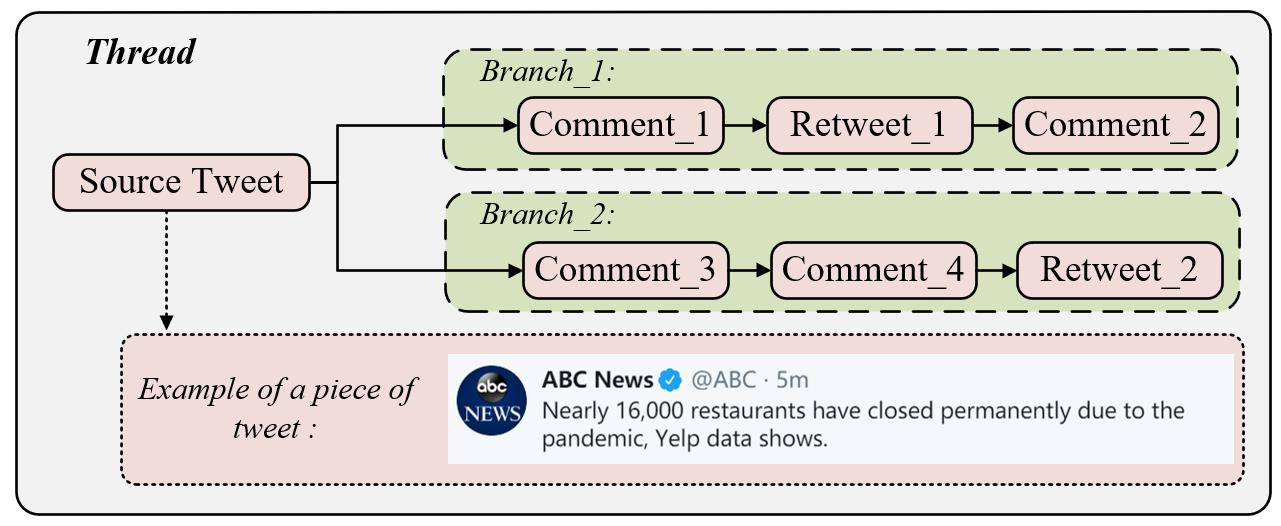
\includegraphics[width = \textwidth]{fig/data_format}
	\caption{An Overview of Social Network Data}
	\label{fig:data_format}
\end{figure}

\subsection{Problem Definition}
\label{sec:problem}
Let $T = \left\{t_1, t_2, ..., t_n \right\}$ denote the set of tweets and each tweet is denoted as $t_n$. Let $C = \left\{c_1, c_2, ... , c_m \right\}$ denote the set of rumor events and $c_m$ denotes a particular rumor event. Each tweet is only assigned with one rumor event. For each given tweet $t_n$, the goal of rumor tracking is to find the most likely relevant event of it. Also, for a testing sample, we will not get any information about its branch or threads in advance. 

In this work, we transfer the binary rumor tracking problem (related/irrelated) into an m-way classification problem. However, source tweets in the dataset are collected by keywords of the event, which causes the source tweets in the same thread are highly similar to each other. We conduct an experiment to train a classifier on source tweets and the classification result even reaches 100\%. Consequently, we should process each tweet independently and cut down its link to source tweet. Only in this way, we can get a convincing result.

\subsection{Aggregated Model}
\label{sec:aggregated_model}
Aggregated model is a mixture model that consists of several different components. For a particular job, several basic models can achieve it. If we combine them, the aggregated performance is usually better than that of a single model. Also, for different types of features, the most suitable classifier is changing. Consequently, using the aggregated model can effectively promote the performance of rumor tracking. 

\subsection{Deep Learning Models for Text Classification}
\label{sec:deeplearning_model} Deep learning models have achieved great success on text classification tasks. In this work, we adopt several different deep learning models as the component of our model. Then we will introduce some of them.

\subsubsection{FastText}
FastText is proposed by BojanowskiGJM17 \cite{DBLP:journals/tacl/BojanowskiGJM17}, which is an extension of the skip-gram model introduced by Mikolov et al. \cite{DBLP:conf/nips/MikolovSCCD13}. The main difference between FastText and skip-gram is that the predictable target of FastText is a classification label rather than a middle word. Also, FastText adopts hierarchical softmax to deal with the large corpus and vocabulary dictionary. With the help of these optimizations, FastText classifies large amounts of texts in a short time.

\subsubsection{TextCNN}
TextCNN uses multiple convolutional filters with different sizes to capture N-gram features. Compared to RNN based models, TextCNN reaches convergence faster due to the parallel computation. Since tweets are usually short text (within 140 words), CNN based models are more suitable than RNN based models for tweets classification. The short texts are sparse on semantic and are usually treated as a bag of words.

\subsubsection{BiLSTM}
BiLSTM is Bi-directional Long Short-Term Memory, which is consisted of a forward-LSTM and a backward-LSTM. BiLSTM can effectively learn the long term dependency of sequential data. So we usually treat it as a evolution of LSTM and it is suitable for text data.

\subsubsection{Naive Bayes}
Naive Bayes is a classical classifier. It assumes that all input variables are independent of each other. Although this model is not complicated, it can achieve a satisfying accuracy with high efficiency. Naive Bayes model is widely adopted in the short text classification problem, showing a pretty good performance. 

\subsubsection{SGD}
SGD is the abbreviation of stochastic gradient descent, which is a optimization strategy in deep learning. SGD updates parameters of a single sample, so SGD works well on dataset with large scale. 

